\section{Turbulence}

\subsection{Overview of Lecture}
Today we will study turbulence - we will first review the idea of a Reynold's number. Then, we will look at the dynamics of turbulence, and see how it is modified in the presence/addition of chiral terms.

The equation we consider is:
\begin{equation}
    \rho[\p_t v_i + v_k \p_k v_i] = - \nabla_i p + \eta \nabla^2 v_i + \eta^0 (\hat{\v{z}} \times \nabla^2 \v{v})_i
\end{equation}
As well as the incompressability condition $\nabla \cdot \v{v} = 0$. Dividing out by $\rho$ we call $\frac{\eta}{\rho} = \nu$ and $\frac{\eta^0}{\rho} = \nu^0$, and so:
\begin{equation}
    \p_t v_i + v_k \p_k v_i = - \frac{1}{\rho}\nabla_i p + \nu \nabla^2 v_i + \nu^0 (\hat{\v{z}} \times \nabla^2 \v{v})_i
\end{equation}
The last term is the 3D generalization of what we wrote down last time, $\eta^0\e_{ij}\p_i \nabla^2v_j$. A key observation - in 3D we no longer have isotropy, because the axis of rotation points in some direction in space (c.f. 2D where the rotation axis can be chosen to point out of the plane). We remark that in 3D, the $\nu^0 (\hat{\v{z}} \times \nabla^2 \v{v})_i$ is not the only term we can have. This is a bit of a stylized/simplified theory, but let us study it and ignore the other possible terms (which do have similar character, e.g. in that they are chiral).

Let us study turbulence as it was understood by Kolmogorov, then see how this $\nu^0 (\hat{\v{z}} \times \nabla^2 \v{v})_i$ term modifies his predictions.

\subsection{Reynold's Number}
It is often to consider equations in dimensionless units; if we measure speed as $\frac{v}{V} = \tilde{v}$ and $\frac{r}{L} = \tilde{r}$ then we can have a dimensionless casting of time as $\frac{t}{\frac{L}{V}} = \tilde{t}$. With this, we define the dimensionless parameter - the \emph{Reynold's Number}:
\begin{equation}
    \text{Re} = \frac{VL}{\nu}
\end{equation}
We want to write down Navier-Stokes in terms of dimensionless parameters as:
\begin{equation}
    \text{Re}\left[\dpd{\tilde{\v{v}}}{\tilde{t}} + (\tilde{\v{v}}\cdot\tilde{\nabla})\tilde{\v{v}}\right] = -\tilde{\nabla}\tilde{p} + \tilde{\nabla}^2\tilde{\v{v}}
\end{equation}
How do we get this? We can write the $\nu$ term as:
\begin{equation}
    \nu\nabla^2 \v{v} = \nu \tilde{\nabla}^2\tilde{\v{v}}\frac{V}{L^2}
\end{equation}
Dividing both sides by $\nu VL^2$ and doing the same rewriting in terms of dimensionless quantities, we get:
\begin{equation}
    \dpd{\v{v}}{t} \to \frac{1}{\nu \frac{V}{L^2}}\frac{1}{\frac{L}{V}}V \dpd{\tilde{\v{v}}}{\tilde{t}} = \frac{VL}{\nu}\dpd{\tilde{\v{v}}}{\tilde{t}} = \text{Re}\dpd{\tilde{\v{v}}}{\tilde{t}}
\end{equation}

There are three limits we consider:
\begin{itemize}
    \item Kolmogorov standard turbulence: $\text{Re} \gg 1$ and $\frac{\eta^0}{\eta} = 0$
    \item Tali will show in guest lecture: $\text{Re} \ll 1$ and $\frac{\eta^0}{\eta} \gg 1$
    \item Odd turbulence: $\text{Re} \gg 1$ and $\frac{\eta^0}{\eta} \gg 1$
\end{itemize}

When $\text{Re} \gg 1$, the $\dpd{\tilde{\v{v}}}{\tilde{t}} + (\tilde{\v{v}}\cdot\tilde{\nabla})\tilde{\v{v}}$ terms are dominant. When $\text{Re} \ll 1$, the $-\tilde{\nabla}\tilde{p} + \tilde{\nabla}^2\tilde{\v{v}}$ are dominant. In the odd turbulent regime, we have that both nonlinearity and chirality ($\nu^0 (\hat{\v{z}} \times \nabla^2 \v{v})$) dominate.



\subsection{Power Spectrum}
The great genius of Kolmogorov starts with a single observation - namely that turbulence should be viewed as a statistical mechanics problem. This is not obvious as Navier-Stokes is determinisitc. But when you have strong non-linearities, an infinitesimally different initial condition can lead to a vastly different outcome. For example with fluid flowing across a sphere, at low Reynolds number (linear) you have smooth flow, while at high velocity (non-linear) you have vortices emerging:

\begin{center}
    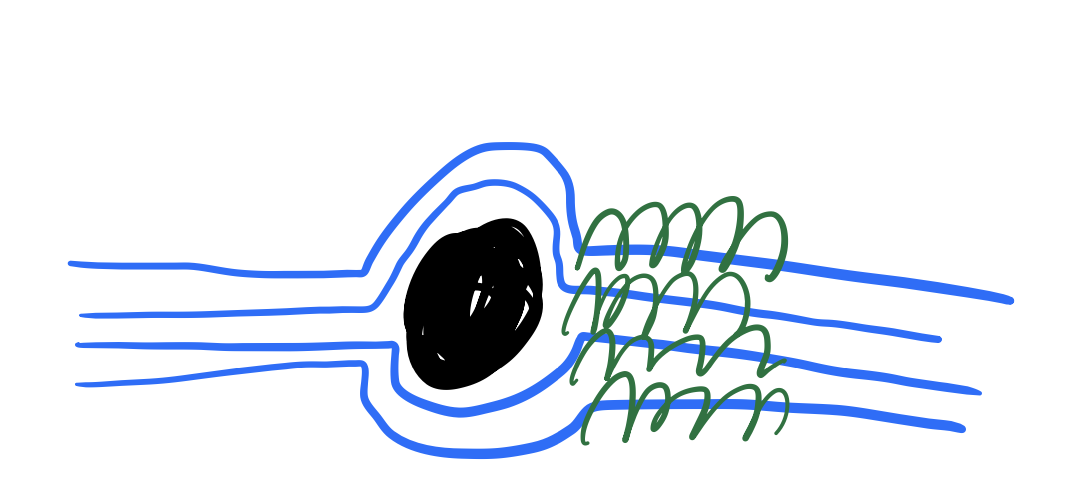
\includegraphics[scale=0.35]{Lectures/Images/lec11-fluidsphere.png}
\end{center}

We consider the power spectrum, a quantity relevant for both theorists and experimentalists. If we assume isotropic, homogenous, and fully developed turbulence:
\begin{equation}
    \v{v}(\v{x}, t) = \left(\frac{2\pi}{L}\right)^3\sum_{\v{k}}\tilde{\v{v}}(k, t)e^{i\v{k} \cdot \v{x}}
\end{equation}
With $\v{k} = (k_x, k_y, k_z) = \frac{2\pi}{L}(n_x, n_y, n_z)$. To find the average of a given observable $A$:
\begin{equation}
    \avg{A}_c = \frac{1}{L^3}\int d^3\v{x}A
\end{equation}
What we will consider is the average of $\frac{v^2}{2}$, the kinetic energy per unit mass. We can compute the average using Parseval's theorem:
\begin{equation}
    \avg{\frac{v^2}{2}}_c = \int d^3\v{k}\frac{1}{2}\abs{\tilde{\v{v}}(k, t)}^2 \equiv \int_0^\infty dk E(k, t)
\end{equation}
The fact that it is homogenous we have already used to going to $k$-space. Isotropy comes in in that in $k$-space there is no preferred direction. Hence we can write:
\begin{equation}
    \int d^3\v{k} = \int 4\pi k^2 dk
\end{equation}
So then the power spectrum (which tells us how the energy is distributes as a function of $k$):
\begin{equation}
    E(k, t) = 4\pi k^2 \frac{1}{2}\abs{\tilde{\v{v}}(k, t)}^2 = 2\pi k^2\abs{\tilde{\v{v}}(k, t)}^2
\end{equation}
If at some time we reach a steady state, then the time-dependence of $E(k, t)$ drops out. Note that the time-invariance we consider here is in a statistical sense; not that the system looks the same at all time, but the average does.

\begin{center}
    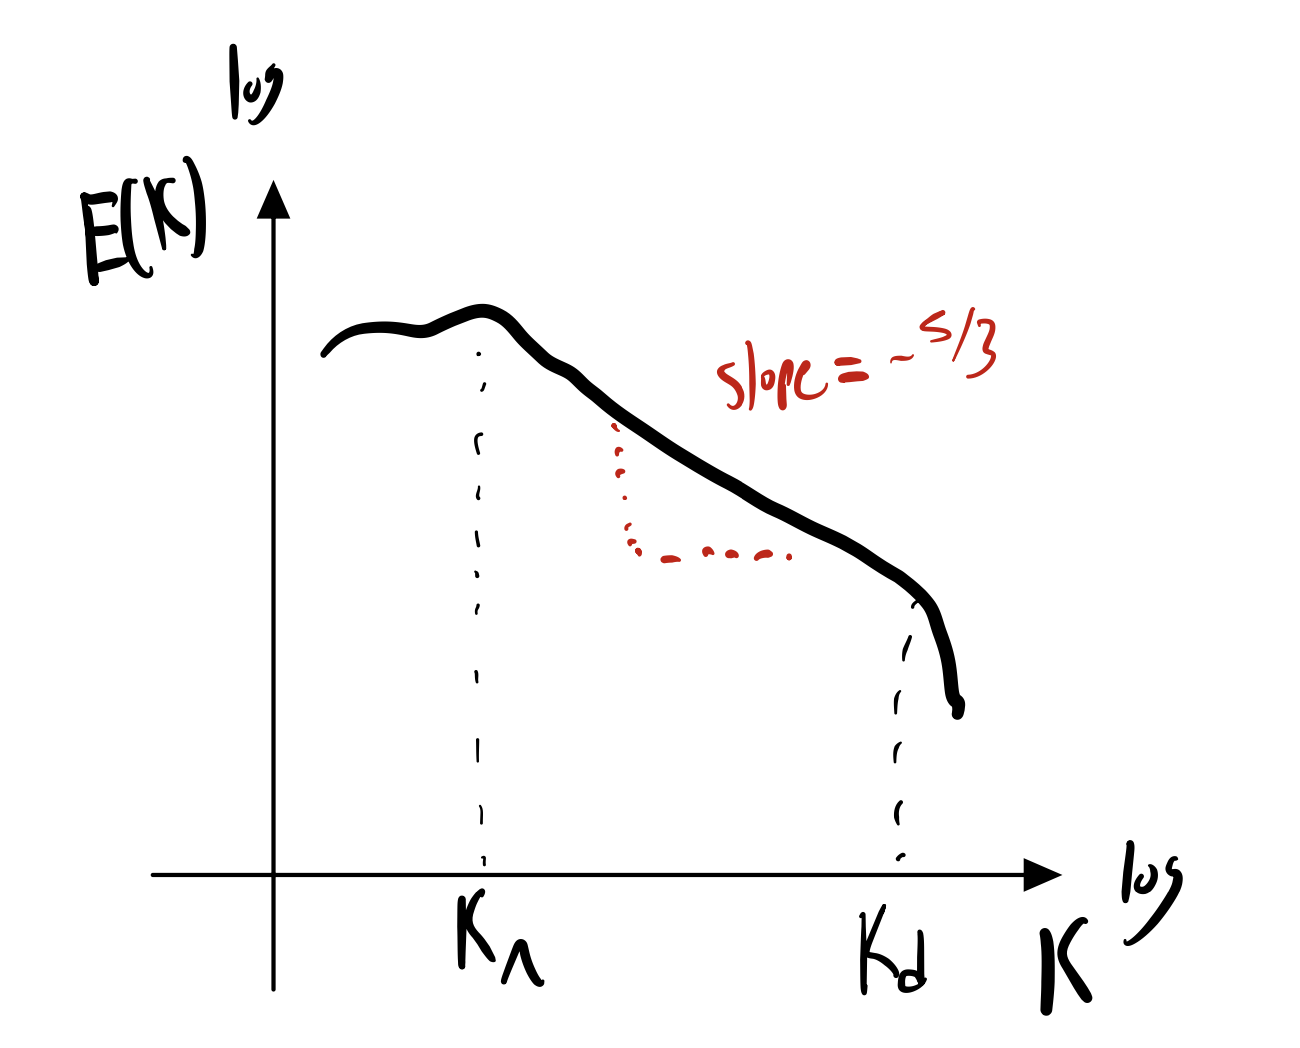
\includegraphics[scale=0.35]{Lectures/Images/lec11-spectrum.png}
\end{center}

Before it was worked out by Kolmogorov, plots/measurements existed that suggested that regimes where $E(k, t)$ becomes time-translation invariant + displays a power law. We can imagine that an experimentalist could measure; to carefully extract the power law, we need to measure something on the length scale of many many decades. We can also use astrophysical/astronomical data to measure this spectrum (albeit with some difficulty, given things like Coriolis effect breaking isotropy). Kolmogorov proved that the slope on this log-log is $-\frac{5}{3}$ under the isotropic, homogenous, fully developed assumption.

\subsection{Power Law Scaling from Vortices and Dimensional Analysis}

In the high Reynolds number scale, interesting things happen - pressure drops out, but so does the second derivative term; we lose dissipation! We consider a vortex/an eddy (we may not be able to see it physically in all systems). We could consider that some external force could be applying a perturbation at a given wavelength. We consider this lengthscale to be $L$/the system size. Since Navier Stokes is energy conserving in the $\text{Re} = \frac{VL}{\nu} \gg 1$ limit, what can happen? Energy cannot go in our out, but energy can redistribute itself, but the eddies can split into eddies of length scale $L$'. But, if it is indeed the case that $\text{Re} = \frac{VL'}{\nu} \gg 1$ even with the new eddies, then these can also potentially split and become smaller vortices. And if the condition still holds then the eddies can continue to split into eddies of $L'', L'''$ and so on. But as the length scale lowers, there may come a point where the size of the vortices/characteristic wavevector becomes such that $\text{Re} = \frac{VL^{(n)}}{\nu} \sim 1$. We call this length scale $L_d$, as it is at this length scale we can start to observe dissipation. It turns out that this self-similar process of splitting of vortices that leads to a power law. In the $E(k)$ plot we had above, the $K_\Lambda = \frac{1}{L}$ corresponding to wavevector of the system size, then we can keep splitting until we reach $K_d = \frac{1}{L_d}$ corresponding to wavevector where we see dissipation, at which point the power law breaks down.

\begin{center}
    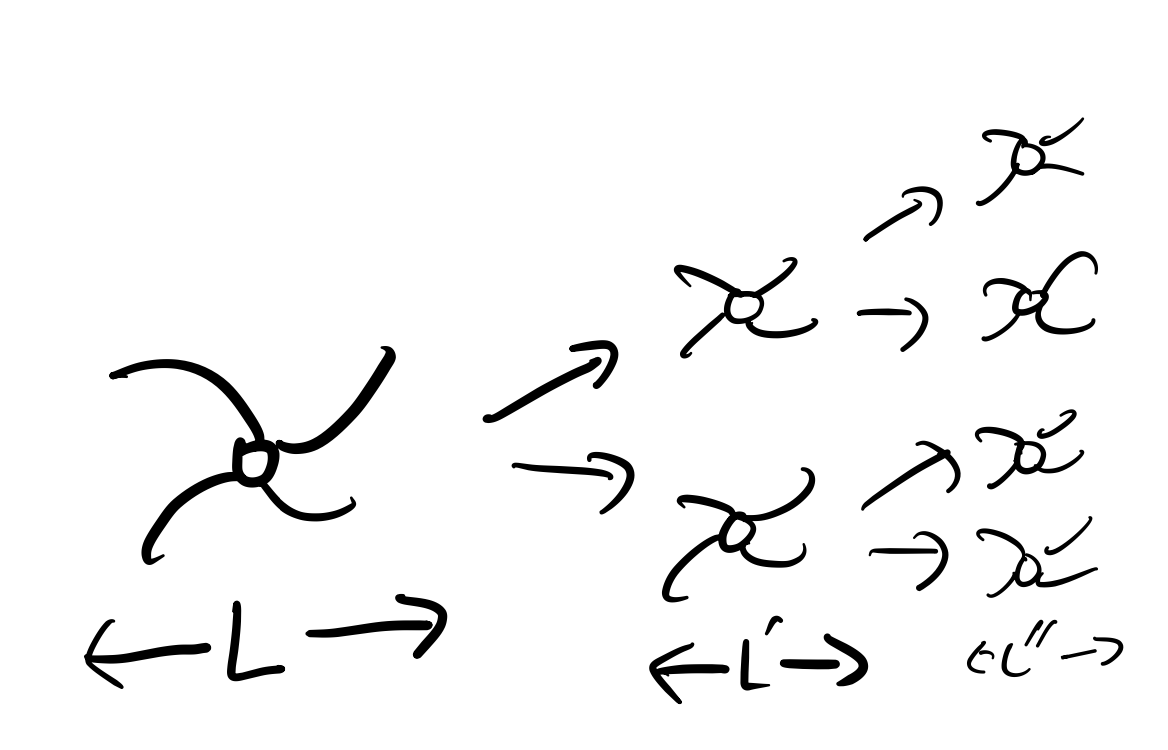
\includegraphics[scale=0.35]{Lectures/Images/lec11-splittingeddy.png}
\end{center}

We can also consider the time scale:
\begin{equation}
    \tau_l \sim \frac{l}{v_l}
\end{equation}
where $l$ is the eddy size and $v_l$ the characteristic velocity. This we call the ``eddy turnover time''. Let's now think about the energy flux that occurs between each scale, e.g. $l \to l/2$. The process that mediates this flux of energy is that the eddy splits. This flux will be equal to the kinetic energy divided by the turnover time:
\begin{equation}
    \Pi_l \sim \frac{v_l^2}{\tau_l} \sim \frac{v_l^3}{l}
\end{equation}
The assumption of Kolmogorov was that this $\Pi_l$ was a constant, until we go to a dissipative scale:
\begin{equation}
    \Pi_l \sim \frac{v_l^3}{l} = \e
\end{equation}
From which:
\begin{equation}
    v_l \sim (\e l)^{1/3}
\end{equation}
\begin{equation}
    \tau_l \sim \e^{-1/3}l^{2/3} \sim \e^{-1/3}k^{-2/3}
\end{equation}
where we have used $\frac{1}{l} \sim k$. The energy per unit mass per eddy is:
\begin{equation}
    \text{KE} \sim \frac{1}{2}v_l^2 \sim E(k)dk
\end{equation}
Hence:
\begin{equation}
    E(k)l^{-1} \sim \left[(\e l)^{1/3}\right]^2 \implies E(k) \sim e^{2/3}l^{5/3} \sim \e^{2/3}k^{-5/3}
\end{equation}
so we reproduce the power-law dependence on $k$ that we expect!

Next time, either we continue with turbulence, but with a caveat - we put the odd viscosity term in, and see what happens to the spectrum. Or, we look at how turbulence changes the analysis of fluid flow around the sphere.